\documentclass{article}

\textwidth=6.5in
\textheight=8.5in
\voffset=-54pt
\oddsidemargin=0in
\evensidemargin=0in
\setlength{\parskip}{8pt}
\setlength{\parindent}{0pt}

\usepackage{amsmath, amssymb}
\usepackage{ifthen}

\usepackage[inline]{enumitem}
\setlist{topsep=0pt, parsep=8pt}

\usepackage[rgb,table]{xcolor}\convertcolorsUfalse
\usepackage{graphicx}

% change hyperref options
\PassOptionsToPackage{hyphens}{url}
\usepackage[bookmarks,colorlinks,linkcolor=black,citecolor=blue,pdfstartview=FitH,urlcolor=blue]{hyperref}
\hypersetup{pdfpagemode=UseNone}
\usepackage{bookmark}

\usepackage{graphicx}
\usepackage{multicol}
\usepackage{framed}
\usepackage{array}

\usepackage{icomma}

\usepackage{pifont}

\usepackage{soul}
\usepackage[normalem]{ulem}

\usepackage{pgfplots}
\pgfplotsset{compat=1.18}  
\pgfplotscreateplotcyclelist{mycolor}{black, blue, red, green!70!black, magenta, purple, cyan, orange }  
\pgfplotsset{
  disabledatascaling,
  cycle list=tikzcolor, 
  axis lines=middle,
  every axis plot/.style={no marks, thick},
  every axis/.style={
    enlarge x limits=false,
    enlarge y limits=auto,
    xlabel style={at={(current axis.right of origin)},anchor=west},
    ylabel style={at={(current axis.above origin)},anchor=south},
    % extra x and y ticks for asymptotes
    extra x tick style={grid=major, grid style={dashed,black}},
    extra y tick style={grid=major, grid style={dashed,black}},
    /pgf/number format/1000 sep={},
  },    
  tick label style = {font=\footnotesize, fill=\currentbgcolor, inner sep=0pt},    
  xticklabel shift=1pt,    
  scaled ticks=false,
  scaled y ticks=false,
  unbounded coords=jump,
  samples=101,
  minor tick length=0,
  scatter/classes={
    open={mark=*,draw=black,fill=white, mark size=2, thin},
    closed={mark=*,draw=black,fill=black, mark size=2, thin}
  },
  width=3in,
}
\pgfplotsset{open/.style={only marks, mark=*, fill=white, thin, mark size=2}}
\pgfplotsset{closed/.style={only marks, mark=*, draw=black, fill=black,
    thin, mark size=2}}
\pgfplotsset{labeled/.style={nodes near coords, only marks, mark=*, draw=black, fill=black, thin, mark size=2, point meta=explicit symbolic}}

\newcommand{\axes}[1][]{
  \begin{tikzpicture}
    \begin{axis}[xtick=\empty, ytick=\empty, ymin=-2, ymax=2,
      xmin=-4.25, xmax=4.25, #1]
    \end{axis}
  \end{tikzpicture}
}
\usepackage{tikz}
\usetikzlibrary{
  matrix,%
  % enables the snake paths
  decorations.pathmorphing,%
  % enables bigger arrows
  decorations.markings,%
  decorations.pathreplacing,%
  decorations.text,%
  calc,%
  patterns,%
  shapes.geometric,%
  arrows,
  decorations.shapes,
  positioning,
  plotmarks,
  intersections
}
\tikzset{>=latex} % sets default arrow type in tikz
\tikzset{font=\normalsize}
\tikzset{mark size=1.5pt, mark options=thin}
\tikzset{pin distance=4pt,
  every pin edge/.style={<-, thin, shorten <= -2pt}}

\interfootnotelinepenalty=10000
\renewcommand{\thefootnote}{(\arabic{footnote})}

\usepackage{multirow, bigdelim}

% change to \usepackage[sols]{handout} to see solutions
\usepackage[]{handout}

\providecommand{\check}{}
\renewcommand{\check}{\ifmmode{\text{ \ding{51} }}\else{\ding{51} }\fi}

\newcommand\iscurrentenumi[1]{%
  \ifthenelse{\equal{#1}{\theenumi}}{}{#1}}
\setenumerate[1]{ref=\#\arabic*}
\setenumerate[2]{ref=\protect\iscurrentenumi{\theenumi}(\alph*)}
\newcommand\enumiiprefix[2]{%
  \ifthenelse{{\equal{#1}{\theenumi}}\AND{\equal{#2}{(\alph{enumii})}}}{}{}%
  \ifthenelse{{\equal{#1}{\theenumi}}\AND{\NOT{\equal{#2}{(\alph{enumii})}}}}{#2}{}%
  \ifthenelse{\equal{#1}{\theenumi}}{}{#1#2}%
}
\setenumerate[3]{ref=\protect\enumiiprefix{\theenumi}{(\alph{enumii})}\roman*}

\newlength{\tipmargin}
\makeatletter

\newdimen\SOUL@dimen %new
\def\SOUL@ulunderline#1{{%
    \setbox\z@\hbox{#1}%
    % \dimen@=\wd\z@
    \SOUL@dimen=\wd\z@ %new
    \dimen@i=\SOUL@uloverlap
    \advance\SOUL@dimen2\dimen@i %\dimen@ exchanged too
    \rlap{%
      \null
      \kern-\dimen@i
      % \SOUL@ulcolor{\SOUL@ulleaders\hskip\dimen@}%
      \SOUL@ulcolor{\SOUL@ulleaders\hskip\SOUL@dimen}% new
    }%
    \unhcopy\z@
  }}

\renewenvironment{framed}{
  \setlength{\tipmargin}{\textwidth-\linewidth}
  \advance\@totalleftmargin-\tipmargin
  \def\FrameCommand{\hspace{\tipmargin}\fbox}%
  \advance\linewidth\tipmargin
  \MakeFramed {\advance\hsize-\width \FrameRestore}%
}
{\endMakeFramed}

\makeatother

\definecolor{purple}{rgb}{0.5,0,1.0}

\usepackage{fancyhdr}
\lhead{\textcolor{white}{This content is protected and may not be shared, uploaded, or distributed.}}
\rhead{}
\rfoot{\vspace*{\fill}\footnotesize\textcopyright{} \emph{Harvard Math Ma}}
\renewcommand{\headrulewidth}{0pt}
\pagestyle{fancy}
\begin{document}

\htitle{25. Derivatives of Exponential Functions}

\begin{problemonly}
  \begin{framed}

You should be able to:
    \begin{itemize}[topsep=0pt,partopsep=0pt,parsep=8pt,itemsep=0pt]
    \item Explain what we mean when we say ``the derivative of an exponential function is proportional to the function itself''.

    \item Explain how the number $e$ is defined in terms of derivatives.

    \item Differentiate $e^{kx}$ where $k$ is any constant.

    \end{itemize}
  \end{framed}
\end{problemonly}

\begin{enumerate}
\item  \label{graph-derivative-of-2^x}

  \begin{enumerate}
  \item
    \begin{problem}
      Sketch the graphs of $f(x) = 2^x$ and $g(x) = 3^x$ on the axes below, and label all intercepts. 
    \end{problem}

    \probonly{\axes[width=3.5in, height=3.5in]}

    \begin{solution}
      \begin{center}
        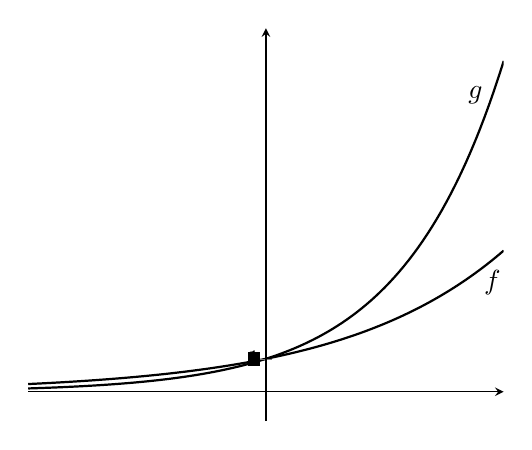
\begin{tikzpicture}
          \begin{axis}[ytick={1}, axis on top, xtick=\empty]
            \addplot[domain=-2.1:2.1] {2^x};
            \addplot[domain=-2.1:2.1] {3^x};
            \node[below] at (2,4) {$f$};
            \node[left] at (2,9) {$g$};
          \end{axis}
        \end{tikzpicture}
      \end{center}
    \end{solution}

  \item

    \note{A common error is for students to draw $f'$ and $g'$ with the same $y$-intercept. It's worth talking about whether this is right.}

    \begin{problem}
      Use your graphs of $f$ and $g$ to sketch graphs of $f'$ and $g'$ on the axes below.
    \end{problem}

    \probonly{\axes[width=3.5in, height=3.5in]}

    \begin{solution}
      \begin{center}
        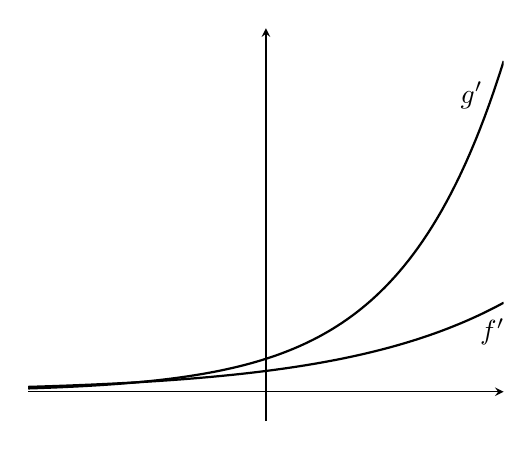
\begin{tikzpicture}
          \begin{axis}[xtick=\empty, ytick=\empty]
            \addplot[domain=-2.1:2.1] {ln(2) * 2^x};
            \addplot[domain=-2.1:2.1] {ln(3) * 3^x};
            \node[below] at (2, 2.77) {$f'$};
            \node[left] at (2, 9.89) {$g'$};
          \end{axis}
        \end{tikzpicture}
      \end{center}
    \end{solution}

  \end{enumerate}

\item 
  \begin{enumerate}
  \item \label{guess-derivative-of-b^x}

    \note{Students looked for patterns in workshop, but they probably didn't guess formulas.}

    In workshop, you came up with something like the following estimates.
    \begin{center}
      \renewcommand{\arraystretch}{1.25}
      \begin{tabular}{rcr}
        \multicolumn{3}{c}{$f(x) = 2^x$} \\
        \hline
        $f'(0)$ & $\approx$ & $ 0.693$ \\
        $f'(1)$ & $\approx$ & $ 1.39$ \\
        $f'(2)$ & $\approx$ & $ 2.77$ \\
        $f'(3)$ & $\approx$ & $ 5.55$ \\
        $f'(4)$ & $\approx$ & $ 11.09$ 
      \end{tabular}
      \hspace{0.5in}
      \begin{tabular}{rcr}
        \multicolumn{3}{c}{$ {g(x) = 3^x}$} \\
        \hline
        $g'(0)$ & $\approx$ & 1.10 \\
        $g'(1)$ & $\approx$ &3.30 \\
        $g'(2)$ & $\approx$ &9.89 \\
        $g'(3)$ & $\approx$ &29.66 \\
        $g'(4)$ & $\approx$ &88.99 
      \end{tabular}
      \hspace{0.5in}
      \begin{tabular}{rcr}
        \multicolumn{3}{c}{$ {h(x) = 10^x}$} \\
        \hline
        $h'(0)$ & $\approx$ &2.30 \\
        $h'(1)$ & $\approx$ & 23.03\\
        $h'(2)$ & $\approx$ & 230.3\\
        $h'(3)$ & $\approx$ &2302.6 \\
        $h'(4)$ & $\approx$ &23026 
      \end{tabular}
    \end{center}

    \begin{problem}[\vfill]
      What patterns did you notice? Can you guess formulas for $h'(x)$, $g'(x)$, and $f'(x)$?
    \end{problem}

    \note{Students may have stated their observations in many different ways. I'll start the discussion with $h'(x)$; each time we increase $x$ by 1, the value of $h'$ is multiplied by 10. That exactly means $h'$ is exponential, and we can write it as $h'(x) = (\approx 2.30) 10^x$ or $h'(x) = h'(0) 10^x$.}

    \begin{solution}
      It appears that, whenever $x$ increases by $1$, $f'(x)$ is multiplied by $2$,
      $g'(x)$ is multiplied by $3$, and $h'(x)$ is multiplied by $10$. This means that
      $f'$, $g'$, and $h'$ are themselves exponential functions: 
      \begin{itemize}
        \item $f'(x) = f'(0) \cdot 2^x \approx (0.693)2^x$,
        \item $g'(x) = g'(0) \cdot 3^x \approx (1.10)3^x$, and
        \item $h'(x) = h'(0) \cdot 10^x \approx (2.3)10^x$.
      \end{itemize}
    \end{solution}

  \item
    \begin{problem}[\stretch{0.25}]
      \check \emph{Consistency check!} Are the formulas you guessed for $f'(x)$ and $g'(x)$ consistent with the graphs you sketched in \ref{graph-derivative-of-2^x}?
    \end{problem}

    \begin{solution}
      Yes. Our graphs are consistent with $f'$ and $g'$ being exponential functions.
    \end{solution}
  \end{enumerate}

\item  Now, let's show that our guess for the derivative of $f(x) = 2^x$ is
  correct!
  \begin{enumerate}

  \item \label{derivative-of-2^x-at-x=0}
    \begin{problem}[0.5in]
      Using the limit definition of the derivative, write a limit that's
      equal to $f'(0)$.
    \end{problem}

    \begin{solution}
      \begin{align*}
        f'(0) &= \lim_{h \to 0} \frac{f(0 + h) - f(0)}{h} \\
        &= \boxed{\lim_{h \to 0} \frac{2^h - 1}{h}}
      \end{align*}
    \end{solution}

  \item

    \note{When I've done this problem in the past, students have seen that they can factor $2^x$ out but then don't recognize how $\dfrac{2^h - 1}{h}$ is related to \ref{derivative-of-2^x-at-x=0}.}

    \begin{problem}[\nstretch{1.65}]
      Using the limit definition of the derivative, write a limit that's equal to $f'(x)$. Does this confirm your guess? (Is there some algebra you can do to rewrite the limit?)
    \end{problem}

    \begin{solution}
      \begin{align*}
        f'(x) &= \lim_{h \to 0} \frac{f(x + h) - f(x)}{h} \\
        &= \boxed{\lim_{h \to 0} \frac{2^{x + h} - 2^x}{h}} \\
        \intertext{We can rewrite this using some algebra:}
        &= \lim_{h \to 0} \frac{2^x (2^h - 1)}{h} \\
        &= \lim_{h \to 0} 2^x \cdot \frac{2^h - 1}{h} \\
        \intertext{Notice that $2^x$ doesn't depend on $h$, so we can
        treat it as a constant and factor it out of the limit:}
        &= 2^x \lim_{h \to 0} \frac{2^h - 1}{h}
        \intertext{As $h \to 0$, $\displaystyle \frac{2^h - 1}{h} \to f'(0)$ by 
        \ref{derivative-of-2^x-at-x=0}, so the previous line becomes:}
        &= 2^x \cdot f'(0)
      \end{align*}
      This is exactly what we guessed in \ref{guess-derivative-of-b^x}. 
    \end{solution}

  \end{enumerate}

\end{enumerate}
\note{Here, I'm just looking for $f'(0) b^x$.}

\begin{framed}
{\bf The Derivative of Exponential Functions (first observation!)}\\
  If $f(x) = b^x$ (where $b$ is a positive constant), then $f'(x) =
  \fitb{1in}{f'(0) b^x}$. 
\end{framed}

\begin{enumerate}[resume]
\item 

  \note{This question is vague, so we'll do it together. We just figured out  that $\frac{d}{dx} \left( 2.5^x \right) = (\text{some constant}) 2.5^x$. The question I really want students to think about is: can we say anything about the size of this constant? I want students to realize that, based on our work with $2^x$ and $3^x$, the constant should be between $0.693$ and $1.099$. That leads us into the question of whether we could find a base $b$ for which the constant is 1.}

  \begin{problem}[\stretch{0.5}]
    What can you say about $\frac{d}{dx} \left( 2.5^x \right)$? 
  \end{problem}

  \begin{solution}
    We know that $\frac{d}{dx} \left( 2.5^x \right)$ will equal some constant times $2.5^x$.
    Moreover, thinking about $2^x$ and $3^x$, this constant should be approximately
    between $0.693$ and $1.10$.
  \end{solution}

\end{enumerate}
\note{Here's a GeoGebra applet that shows $b^x$: \url{https://www.geogebra.org/m/snmmxqvw}}

\begin{framed}
  \textbf{The number $\bm{e}$}. We define $e$ to be the number $b$ such that the slope of $y = b^x$ at $x = 0$ is $\vphantom{\dfrac{1}{1}}$\fitb{0.25in}{1}. 
\end{framed}

\begin{enumerate}[resume]
\item  
  \begin{enumerate}

  \item
    \begin{problem}[\vfill]
      What does the definition of $e$ tell you about the derivative of $e^x$?
    \end{problem}

    \begin{solution}
      If $f(x) = e^x$, we've already seen that $f'(x) = f'(0) e^x$. But $f'(0)$ is the slope of $y = e^x$ at $x = 0$, and this slope is 1 because that's exactly how we defined $e$! So, $f'(x) = e^x$. 

    \end{solution}  

  \item

    \note{Here, I just want students to recognize that $e$ is between 2 and 3. They'll come up with a better approximation in the homework (\#3).}

    \begin{problem}[\stretch{0.5}]
      What can you say about the size of $e$?
    \end{problem}

    \begin{solution}
      See \href{https://people.math.harvard.edu/~jjchen/mathma/docs/homework/PS24.html}{Problem Set 24}, {{{{\#3}}(b)}}. 
    \end{solution}

  \end{enumerate}

\item  \label{deriv-of-e^3x}

  Now, let's find the derivative of $g(x) = e^{3x}$!

  \begin{enumerate}
  \item \label{deriv-of-e^3x-a}

    \note{The point of rewriting $g(x) = b^x$ is just so that we can use the fact that then $g'(x) = g'(0) b^x = g'(0) e^{3x}$.}

    \begin{problem}[\stretch{0.5}]
      $g(x) = e^{3x}$ can be written as $b^x$ for what value of $b$? What does that tell you about $g'(x)$? 
    \end{problem}

    \begin{solution}
      $\left( e^{3x} \right) = \left( e^3 \right)^x$. Since $g(x)$ can be written as $g(x) = b^x$, we know that $g'(x) = g'(0) b^x = g'(0) \left( e^3 \right)^x = g'(0) e^{3x}$. 
    \end{solution}

  \item \label{deriv-of-e^3x-at-0}
    \begin{problem}[\stretch{1.25}]
      Let $f(x) = e^x$. How does the graph of $g(x)$ relate to the graph of $f(x)$? What does that tell you about how $g'(0)$ relates to $f'(0)$?
    \end{problem}

    \begin{solution}
      Since $g(x) = f(3x)$, the graph of $g$ is the graph of $f$ stretched horizontally by a factor of $\frac{1}{3}$. That makes the tangent line to $g$ at $x = 0$ have a slope that's 3 times the slope of the tangent line to $f$ at $x = 0$, so $g'(0) = 3 f'(0)$. Of course, we defined $e$ so that $f'(0) = 1$, so that tells us $g'(0) = 3$.
    \end{solution}

  \item
    \begin{problem}[\newpage]
      What's $g'(x)$? (We can also confirm this using the Chain Rule!)
    \end{problem}

    \begin{solution}
      In \ref{deriv-of-e^3x-a}, we found that \[g'(x) = g'(0) e^{3x}.\] In \ref{deriv-of-e^3x-at-0}, we found that $g'(0) = 3$, so
      \[ g'(x) = 3 e^{3x}.\]
    \end{solution}

  \end{enumerate}

\end{enumerate}
\begin{framed}
 \textbf{ The Derivative of $e^{x}$ and $e^{kx}$}\\
  $\displaystyle \frac{d}{dx} e^x = \fitb{0.5in}{e^x}$.  More generally, for any
  constant $k$, $\displaystyle \frac{d}{dx} e^{kx} = \fitb{0.75in}{ke^{kx}}$.
\end{framed}

\begin{enumerate}[resume]
\item  \emph{General exponential functions.}

  \begin{enumerate}

  \item

    \note{Here, $j'(x) = (\approx 1.099) j(x)$, so $j(x)$ is a multiple of $j(x)$, but that multiple isn't $j'(0)$.}

    \begin{problem}[\stretch{2}]
      We've now seen that $\frac{d}{dx} \left( 2^x \right) = (\approx
      0.693) 2^x$, $\frac{d}{dx} \left( 3^x \right) = (\approx 1.099)
      3^x$, and $\frac{d}{dx} \left( 10^x \right) = (\approx 2.305)
      10^x$.

      If $j(x) = 7 \cdot 3^x$, what's $j'(x)$?  How does it relate to
      $j(x)$?
    \end{problem}

    \begin{solution}
      By the Constant Multiple Rule, $j'(x) = 7 \frac{d}{dx}(3^x) = 7(\approx\!1.099)3^x$,
      which we can rewrite as $(\approx\!1.099) \cdot j(x)$. Notice that $j'(0)$ is 
      not approximately $1.099$.
    \end{solution}

  \item \label{exponential-function-derivative-proportional-to-function}

    \note{I just want to summarize this as $j'(x)$ is a constant times $j(x)$. What the constant is isn't important.} 

    \begin{problem}[\stretch{0.5}]
      Generalize: if $j(x)$ is any exponential function $j(x) = C \cdot b^x$, how does $j'(x)$ relate to $j(x)$?
    \end{problem}

    \begin{solution}
      $j'(x)$ is some constant times $j(x)$.
    \end{solution}

  \end{enumerate}

\end{enumerate}
\probonly{
  \begin{framed}
    We say that two functions $A(x)$ and $B(x)$ are \ul{proportional} to each other if one is a constant multiple of the other; in other words,
    $$A(x) = kB(x)$$
    for some constant $k$ (called the {\it constant of proportionality}). So, \textbf{\textsf{the derivative of an exponential function is proportional to the function itself!}} Moreover, exponential functions are the \uline{only} functions with this property!
  \end{framed}
}

\begin{enumerate}[resume]
\item 

  Find the derivative of each function. 
  \begin{enumerate}
  \item
    \begin{problem}[\vfill\newpage]
      $f(x) = \dfrac{x^2 e^{3x}}{7}$
    \end{problem}

    \begin{solution}
      Let's first rewrite the function as $f(x) = \frac{1}{7}x^2e^{3x}$. Now
      we can use the Product Rule.
      \begin{align*}
        \frac{d}{dx} \tfrac{1}{7}x^2e^{3x} &= 
        \tfrac{1}{7}\left[\left(\tfrac{d}{dx}x^2\right) (e^{3x})
        + (x^2)\left(\tfrac{d}{dx}e^{3x}\right)\right] \\
        &= \boxed{\tfrac{1}{7} \left[(2x)(e^{3x}) + (x^2)(3e^{3x})\right]}
        \intertext{Optionally, we can factor out $e^{3x}$ to simplify.}
        &= \tfrac{1}{7}e^{3x}(2x+3x^2).
      \end{align*}
    \end{solution}

  \item
    \begin{problem}[\vfill]
      $f(x) = \dfrac{e^{5x} + 1}{e^{2x}}$
    \end{problem}

    \begin{solution}
      Let's first rewrite the function as $f(x) = \frac{e^{5x}}{e^{2x}} + \frac{1}{e^{2x}} =
      e^{3x} + e^{-2x}$. Now we can apply the derivative rule that we just found.
      \begin{align*}
        f'(x) &= \frac{d}{dx}(e^{3x} + e^{-2x}) \\
        &= \frac{d}{dx}e^{3x} + \frac{d}{dx}e^{-2x} \\
        &= \boxed{3e^{3x} - 2e^{-2x}}.
      \end{align*}
    \end{solution}

  \item
    \begin{problem}[\vfill]
      $f(x) = \dfrac{e^{2x}}{e^{5x} + 1}$
    \end{problem}

    \begin{solution}
      To differentiate this function, we can use the Quotient Rule.
      \begin{align*}
        f'(x) &= \frac{d}{dx}\left(\frac{e^{2x}}{e^{5x} + 1}\right) \\
        &=\frac{(\tfrac{d}{dx}e^{2x})(e^{5x}+1)-(e^{2x})(\tfrac{d}{dx}(e^{5x}+1))}{(e^{5x}+1)^2} \\
        &= \boxed{\frac{(2e^{2x})(e^{5x}+1)-(e^{2x})(5e^{5x})}{(e^{5x}+1)^2}}.
      \end{align*}
    \end{solution}

  \end{enumerate}

\item  

  Let $f(x) = 2ex - e^{2x}$.

  \begin{enumerate}
  \item
    \begin{problem}[\nstretch{3}]
      Where is $f$ increasing? Where is $f$ decreasing? 
    \end{problem}

    \begin{solution}
      First, we need to find $f'(x)$. Using our derivative rules, we have $f'(x)=2e-2e^{2x}$.
      Now we need to make a sign chart for $f'(x)$. Since $f'(x)$ is never undefined,
      we just need to look for where $f'(x)=0$.
      \begin{align*}
          2e - 2e^{2x} &= 0 \\
          2e &= 2e^{2x} \\
          e &= e^{2x} \\
          1 &= 2x \\
          x &= \tfrac{1}{2}. 
      \end{align*}
      Testing values on either side of $x=\frac{1}{2}$, we find that the sign chart looks
      like this.
       \begin{center}
        \begin{tikzpicture}
          \draw[<->] (-2,0) -- (2, 0);
          \node[left] at (-2,0) {$f'(x)$};
          \draw[shift={(0,0)},color=black] (0pt,3pt) -- (0pt,-3pt) node[below] 
            {$\frac{1}{2}$};
          \node[circle, fill=black, inner sep=2pt] at (0,0) {};
          \node[above] at (-1,0) {$+$};
          \node[above] at (1,0) {$-$};
        \end{tikzpicture}
      \end{center}
      Based on the sign chart, $f$ is increasing on the interval $(-\infty, \frac{1}{2})$
      and decreasing on the interval $(\frac{1}{2}, \infty)$. 
    \end{solution}

  \item
    \begin{problem}[\vfill]
      Where is $f$ concave up? Where is $f$ concave down? 
    \end{problem}

    \begin{solution}
      We need to find $f''(x)$. Using derivative rules, $f''(x)=-4e^{2x}$. This is always
      negative, i.e. the sign chart for $f''(x)$ looks like this.
      \begin{center}
        \begin{tikzpicture}
          \draw[<->] (-2,0) -- (2, 0);
          \node[left] at (-2,0) {$f''(x)$};
          \node[above] at (0,0) {$-$};
        \end{tikzpicture}
      \end{center}
      Therefore $f$ is concave down on $(-\infty, \infty)$. 
    \end{solution}

  \item
    \begin{problem}[\stretch{0.5}]
      Does $f$ achieve a global maximum on $(-\infty, \infty)$? If so, what is the maximum value? How about a global minimum?
    \end{problem}

    \begin{solution}
      Yes, $f$ achieves a global maximum on $(-\infty, \infty)$, at $x=\frac{1}{2}$. 
      The maximum value is $f(\frac{1}{2}) = 2e(\frac{1}{2}) - e^{2(1/2)} = e-e = 0$.
      There is no global minimum value, as $f$ increases on $(-\infty, \frac{1}{2})$ and
      decreases on $(\frac{1}{2}, \infty)$. 
    \end{solution}

  \item
    \begin{problem}[\vfill]
      Sketch a rough graph of $f$. 
    \end{problem}

    \begin{solution}
      We know that $f$ is increasing on $(-\infty, \frac{1}{2})$, decreasing on 
      $(\frac{1}{2}, \infty)$, concave down on $(-\infty, \infty)$, and has a global
      maximum at $(\frac{1}{2}, 0)$. The graph looks like this.
      \begin{center}
        \begin{tikzpicture}
          \begin{axis}[xtick=\empty, ytick=\empty]
            \addplot[domain=-1.5:1.5] {2*e*x - e^(2*x)};
          \end{axis}
        \end{tikzpicture}
      \end{center}
    \end{solution}

  \item

    \note{We can use the graph to answer these (the concavity makes the end behavior unambiguous). We can do $\displaystyle \lim_{x \to -\infty} f(x)$ algebraically, but we don't yet know enough to do $\displaystyle \lim_{x \to \infty} f(x)$ algebraically.}

    \begin{problem}[\stretch{0.5}]
      What are $\displaystyle \lim_{x \to -\infty} f(x)$ and $\displaystyle \lim_{x \to \infty} f(x)$?
    \end{problem}

    \begin{solution}
      Based on the graph, $\lim\limits_{x\to-\infty}f(x) = -\infty$, and 
      $\lim\limits_{x\to\infty} f(x) = -\infty$.
    \end{solution}

  \end{enumerate}

\end{enumerate}
\end{document}
